\documentclass[11pt]{article}
\usepackage{blindtext}
\usepackage{enumitem}
\usepackage{minted}
%Gummi|065|=)
\title{\textbf{Decommerce}}
\author{Mirco Romagnoli\\
		Giorgio Fiori}
\date{\today}
\usepackage{graphicx}
\begin{document}

\maketitle

\section{Introduzione}

Il progetto \`e un portale di e-commerce che permette a diversi venditori di mettere in vendita prodotti delle categorie:
\begin{itemize}
 \item Abbigliamento
 \item Elettronica
 \item Giardinaggio
 \item Giocattoli
 \item Libri
 \item Musica
 \item Orologi
 \item Sport
 \item Strumenti Musicali
\end{itemize}

\section{Funzionalit\`a}
Il sito permette di mettere in vendita dei prodotti e permette di scrivere recensioni di prodotti e venditori, inoltre il sistema fornisce suggerimenti su prodotti simili a quelli visualizzati agli utenti tramite un sistema basato su tags. \\
Tutti gli utenti registrati devono fornire una mail, uno username e una password.\\
Il sito divide i suoi utenti in tre tipologie:
\begin{description}
	\item [Venditori] possono mettere in vendita i prodotti, devono fornire un nome per il loro "Negozio", il nome deve essere unico
	\item [Compratori] possono comprare e lasciare recensioni su prodotti e venditori, al momento della registrazione devono fornire la nazionalit\`a e l'indirizzo
	\item [Utenti non registrati] possono navigare il sito senza per\`o comprare i prodotti o visualizzare le recensioni
\end{description}

\section{Logica}
\subsection{Applicazione}
La logica del progetto \`e strutturata su un'unica applicazione (esclusa quella di amministrazione), in questo modo viene impiegato un singolo modello.
L'applicazione sfrutta anche un context processor contenuto nel file\\ \texttt{decommerce/context\_processor.py}, questo file si occupa di creare un contesto di base contenente: le categorie in ordine alfabetico, due booleani che identificano l'utente come compratore o venditore e, nel caso l'utente sia un compratore, il carrello; queste informazioni sono utilizzate in tutti i template, di conseguenza \`e utile richiamarlo ad ogni richiesta per rendere pi\`u pulito il codice delle view.\\
In ogni view il context viene poi aggiornato per inserire gli elementi che serviranno al template, vengono inoltre fatti tutti i controlli necessari (richieste POST o GET, controlli sul login ecc.).\\
Gli utenti vengono divisi in due gruppi con differenti permessi, al momento della registrazione la view inserir\`a l'utente registrato nel gruppo richiesto, in questo modo il sistema potr\`a permettere o negare l'accesso a determinate pagine ad un utente.\\
I template derivano tutti dal template \texttt{base.html} che determina
lo stile generale delle pagine e fornisce alcuni script di base che possono essere utilizzati su diversi template, essi poi deriveranno da altri template che svolgono specifici compiti oppure andranno a modificare la visualizzazione della pagina tramite javascript.

\subsection{Modello}
\makebox[\textwidth]{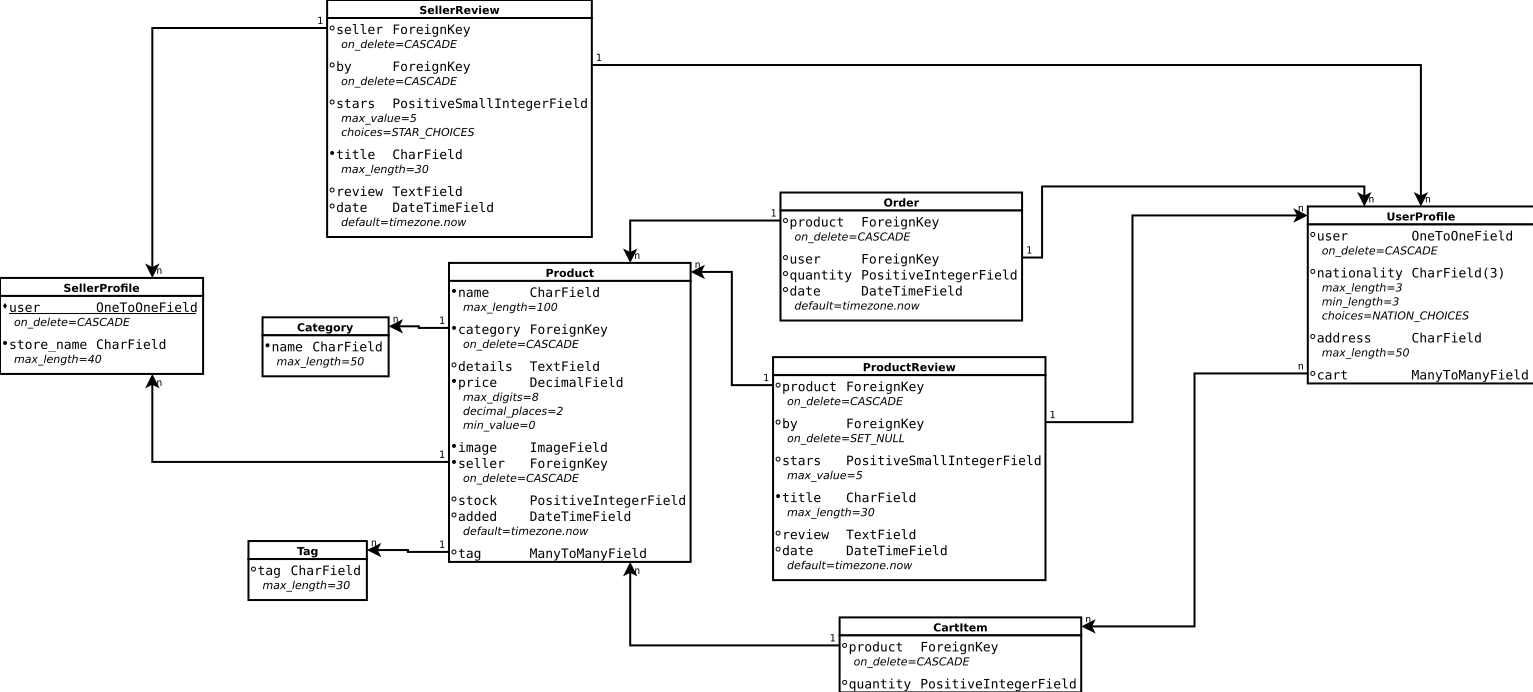
\includegraphics[width=\paperwidth - 50pt]{img/db_diagram.pdf}}\\ \begin{center}{\emph{Schema del modello}}\end{center}
Ogni prodotto pu\`o contenere diversi tag, questi serviranno per determinare quanto due prodotti si assomigliano (due prodotti con molti tag in comune si assomiglieranno di pi\`u rispetto a due prodotti che ne hanno pochi), si \`e anche deciso di mettere tutti i tag in una tabella per permettere di ottenere tutti i tag in una sola query.\\
Le varie date contenute nel modello possono indicare anche un momento nel futuro, sar\`a poi compito delle view filtrare i prodotti o le recensioni con data nel futuro.

\subsection{Templates}
\makebox[\textwidth]{\includegraphics[width=\paperwidth - 50pt]{img/template_tree.pdf}}\\ \begin{center}{\emph{Albero dei template}}\end{center}
Il template \texttt{product\_show.html} viene usato quando si deve mostrare una lista di prodotti, essi vengono passati tramite la variabile \texttt{product\_list} e verranno visualizzati tramite una tabella.

\section{Struttura}
\subsection{Struttura generale}
\makebox[\textwidth]{\includegraphics[width=\paperwidth - 50pt]{img/index.png}}\\ \begin{center}{\emph{Homepage}}\end{center}
La homepage mostra i dieci prodotti pi\`u recenti di qualsiasi categoria, a sinistra si possono esplorare le varie categorie, mentre in alto si trovano in ordine: la barra di ricerca, il pulsante di login e il pulsante per la registrazione. Nel caso un utente sia registrato, sotto alla scritta "Decommerce" si potr\`a leggere un messaggio di benvenuto che mostra lo username dell'utente loggato.\\

\makebox[\textwidth]{\includegraphics[width=\paperwidth - 50pt]{img/topbar.png}}\\ \begin{center}{\emph{Barra superiore}}\end{center}
Se l'utente appartiene al gruppo dei "Buyer" allora ci sar\`a anche un pulsante per mostrare il carrello.
Quando non ci si trova nella homepage allora verr\`a mostrato anche un pulsante per tornare alla home. I due pulsanti centrali servono per effettuare il logout e per visualizzare il profilo dell'utente, vengono mostrati in qualsiasi caso.

\subsection{Profili utente}
\makebox[\textwidth]{\includegraphics[width=\paperwidth - 50pt]{img/sellerProfile.png}}\\ \begin{center}{\emph{Profilo del venditore}}\end{center}
In questa pagina il venditore pu\`o mettere in vendita i propri prodotti e accedere alle statistiche individuali per ogni prodotto.

\makebox[\textwidth]{\includegraphics[width=\paperwidth - 50pt]{img/sellerProfileVisitor.png}}\\ \begin{center}{\emph{Profilo del venditore visto da un compratore}}\end{center}
Il profilo di un venditore se visto tramite l'account di un compratore appare in questo modo, l'utente pu\`o solamente visualizzare le recensioni o scriverne una, se ha gi\`a scritto una recensione la form viene disabilitata.

\makebox[\textwidth]{\includegraphics[width=\paperwidth - 50pt]{img/buyerProfile.png}}\\ \begin{center}{\emph{Profilo di un compratore}}\end{center}
Il profilo di un compratore pu\`o essere visualizzato solo da s\`e stesso, un venditore non pu\`o visualizzarlo e nemmeno un altro compratore. Qui si pu\`o: gestire il carrello, visualizzare i propri ordini e modificare i dati personali. Se l'utente ha comprato un prodotto ma non ha ancora recensito il prodotto o il venditore allora gli verr\`a notificato.

\makebox[\textwidth]{\includegraphics[width=\paperwidth - 50pt]{img/search.png}}\\ \begin{center}{\emph{Risultato di una ricerca}}\end{center}
I risultati di una ricerca vengono raccolti cercando il testo della query all'interno di: nome, dettagli, nome dello store e i tag. I risultati della ricerca potranno essere poi filtrati per diversi termini, cercando anche prodotti che hanno specifici tag.

\end{document}
